\documentclass[11pt]{article}

\usepackage{comment} % enables the use of multi-line comments (\ifx \fi) 
\usepackage[a4paper,margin=1cm]{geometry}
\usepackage[utf8]{inputenc}
\usepackage[ngerman]{isodate}
\usepackage{gensymb}
\usepackage{graphicx}
\usepackage{booktabs}% http://ctan.org/pkg/booktabs
\usepackage{tabularx}
\usepackage{ltablex} % Longtables with tabularx
\usepackage[x11names]{xcolor}
\usepackage{amsmath}
\usepackage{amssymb}
\usepackage{amsthm}
\usepackage{array}
\usepackage{wrapfig}
\usepackage{subcaption}
\usepackage{csquotes}
\usepackage{lscape}
\usepackage{geometry}
\usepackage{multicol}
\usepackage{bm}
\usepackage{enumitem}
\usepackage{hyperref}
\usepackage{mdframed}
\usepackage{scalerel}
\usepackage{stackengine}
\usepackage{mathtools}
\usepackage{pdfpages}

% Code highlighting
\usepackage{minted}
\surroundwithmdframed{minted}

% Be able to caption equations and float them in place
\usepackage{float}

% Bibliography & citing
\usepackage[
	backend=biber,
	style=apa,
	bibstyle=apa,
	citestyle=apa,
	autolang=langname,
	sortlocale=en_UK
]{biblatex}
\addbibresource{Bibliography.bib}
% print the whole bibliography
\nocite{*}

\newmdtheoremenv{theorem}{Theorem}

\theoremstyle{definition}
\newmdtheoremenv{definition}{Definition}[section]


\geometry{a4paper, margin=2.4cm}

\newcommand\equalhat{\mathrel{\stackon[1.5pt]{=}{\stretchto{\scalerel*[\widthof{=}]{\wedge}{\rule{1ex}{3ex}}}{0.5ex}}}}
\newcommand\defeq{\mathrel{\overset{\makebox[0pt]{\mbox{\normalfont\tiny def}}}{=}}}
\newcolumntype{C}{>{\centering\arraybackslash}X}

\newcommand*\samplemean[1]{\overline{#1}}
\newcommand*\ev[1]{\mathrel{\text{E}\left[#1\right]}}
\newcommand*\R{\mathbb{R}}
\newcommand*\Z{\mathbb{Z}}
\newcommand*\N[1]{\mathcal{N}\left(#1\right)}
\newcommand*\Likelihood{\mathcal{L}}
\newcommand*\diff{\mathop{}\!\mathrm{d}}
\newcommand*\Diff[1]{\mathop{}\!\mathrm{d^#1}}
\newcommand*\Exp[1]{\mathop{\text{Exp}}\left(#1\right)}
\newcommand*\Cov[1]{\mathop{\text{Cov}}\left(#1\right)}
\newcommand*\Cor[1]{\mathop{\text{Cor}}\left(#1\right)}
\newcommand*\Var[1]{\mathop{\text{Var}}\left(#1\right)}

\DeclarePairedDelimiter\abs{\lvert}{\rvert}
\DeclarePairedDelimiter\norm{\lVert}{\rVert}

\setcounter{tocdepth}{3}
\setcounter{secnumdepth}{3}

\graphicspath{{./img/}}



\begin{document}
	
\title{Ethics HS21}
\author{Pascal Baumann\\pascal.baumann@stud.hslu.ch}
\maketitle

For errors or improvement raise an issue or make a pull request on the \href{https://github.com/KilnOfTheSecondFlame/mse_summaries}{github repository}.

\tableofcontents
\newpage

\section{Introduction}

\subsection{The Need for Ethics}
The fundamental question of ethics is \textquotedblleft What should I do\textquotedblright. This question reflects freedom and commitment, but an individual should also
\begin{itemize}[label=-, nosep]
	\item be good
	\item behave well
	\item strive for good conditions
\end{itemize}

\noindent
Ethics can help in this aspect in the following way
\begin{itemize}
	\item As a guideline for human action
	\item Ethical debates are advice for laws
\end{itemize}

\begin{figure}[tbh]
	\centering
	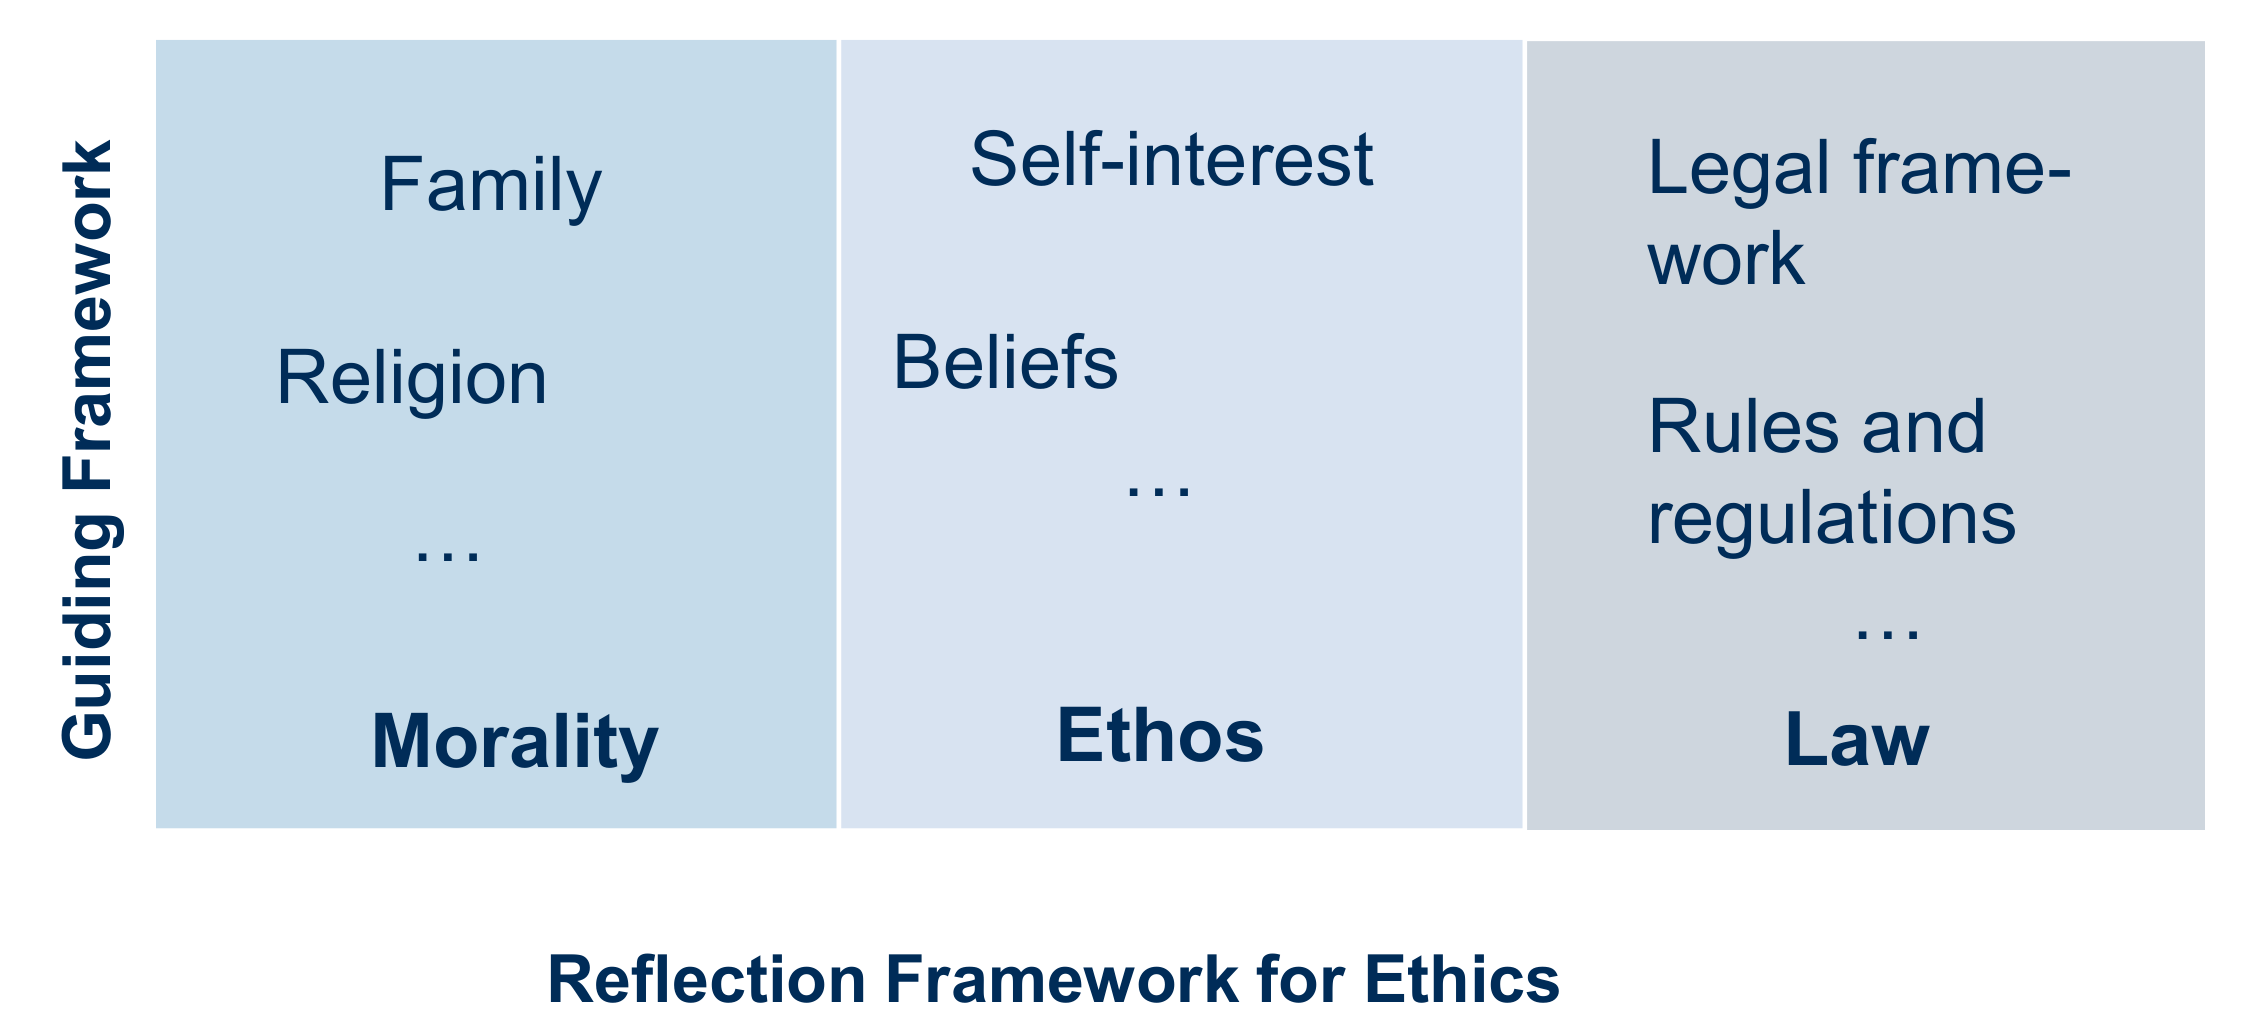
\includegraphics[width=0.8\linewidth]{img/ethics_frame}
	\caption{The different frames an ethical question can arise in}
	\label{fig:ethicsframe}
\end{figure}

\begin{figure}[tbh]
	\centering
	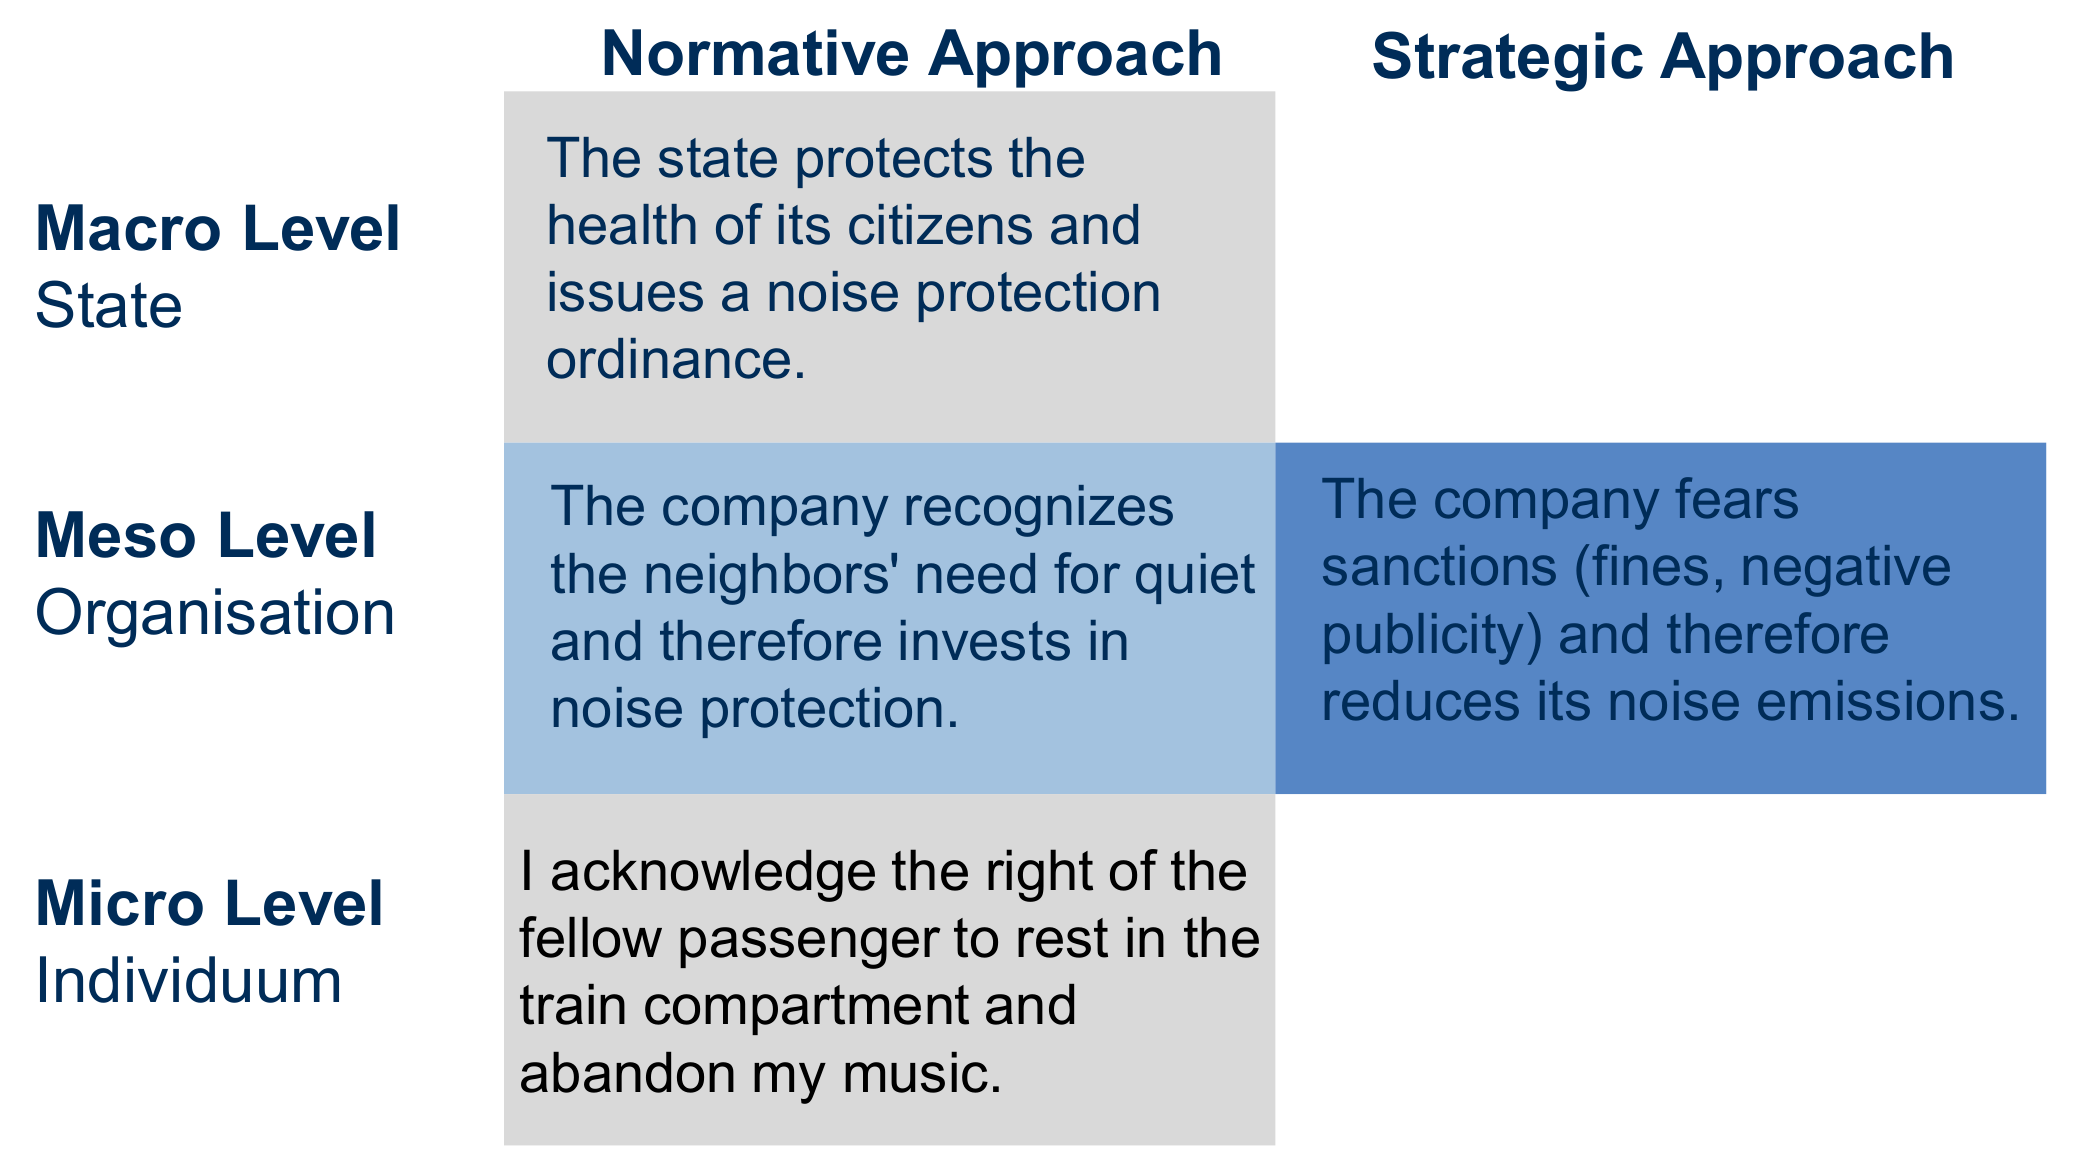
\includegraphics[width=0.6\linewidth]{img/ethics_approach}
	\caption{Normative and Strategic Approaches broken down on Macro-, Meso- and Micro-Level}
	\label{fig:ethicsapproach}
\end{figure}

\begin{definition}
	\textbf{Morality} is what at a certain time in a certain society is generally considered good and desirable or evil and forbidden as an action, condition, or attitude is collectively called the prevailing morality \parencite{gobel2013unternehmensethik}.
	
	But morality only means that a system of norms claims to be valid, not that it is justified.
\end{definition}

\begin{definition}
	\textbf{Law} can be understood as a system of positive coercive norms applying to individuals, including sanctions associated with them.
\end{definition}

\begin{definition}
	\textbf{Ethos} refers to a subject who recognizes a certain morality as a requirement for his or her actions and to actions that are consistently marked by recognition.
\end{definition}

\begin{center}
	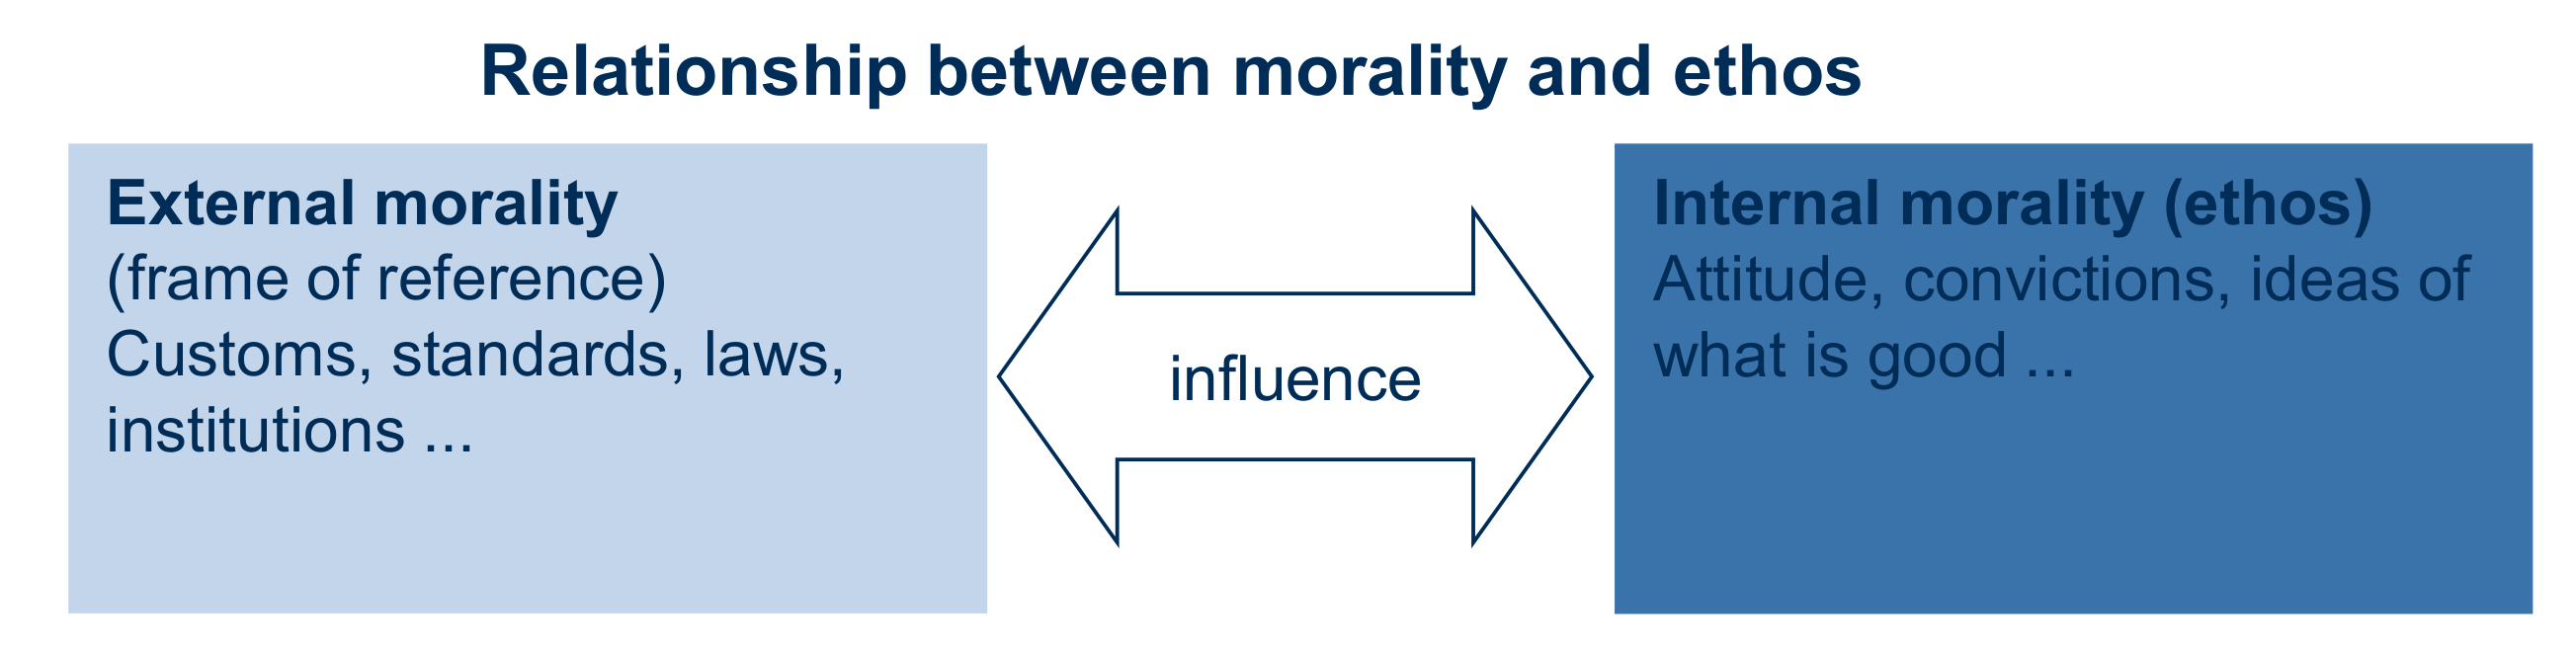
\includegraphics[width=0.8\linewidth]{img/ethos}
\end{center}

\begin{definition}
	\textbf{Ethics} in general can be described as the teaching or the science of morals and ethos.
\end{definition}

Ethics analyzes the answers provided by different forms of morality to questions on what one should do, one's duties and rights, what can be considered good and bad, and what is right or wrong.

\begin{figure}[tbh]
	\centering
	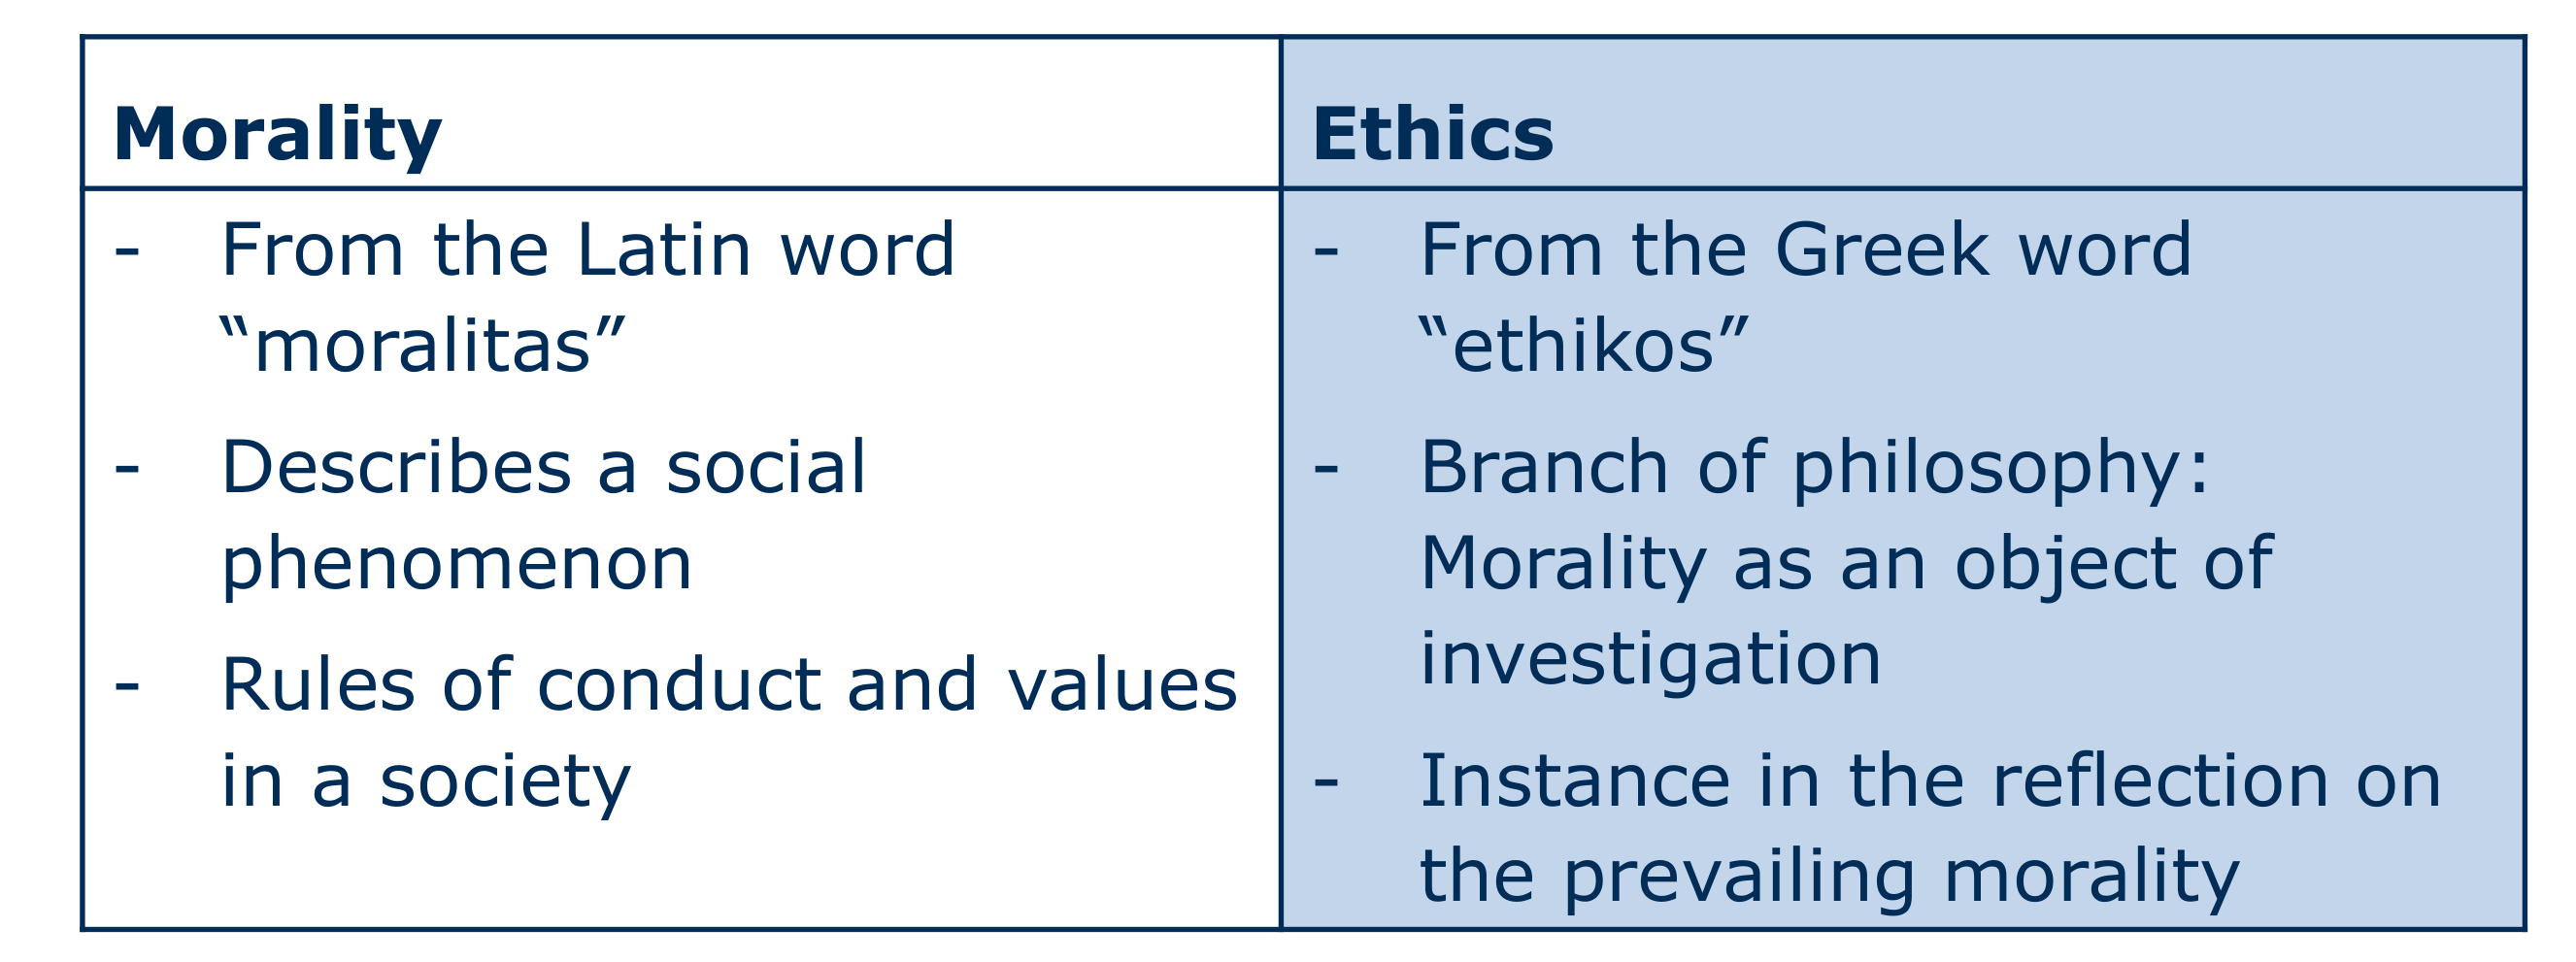
\includegraphics[width=0.6\linewidth]{img/morality_ethics}
	\caption{Comparison between morality and ethics}
	\label{fig:moralityethics}
\end{figure}

\begin{figure}[tbh]
	\centering
	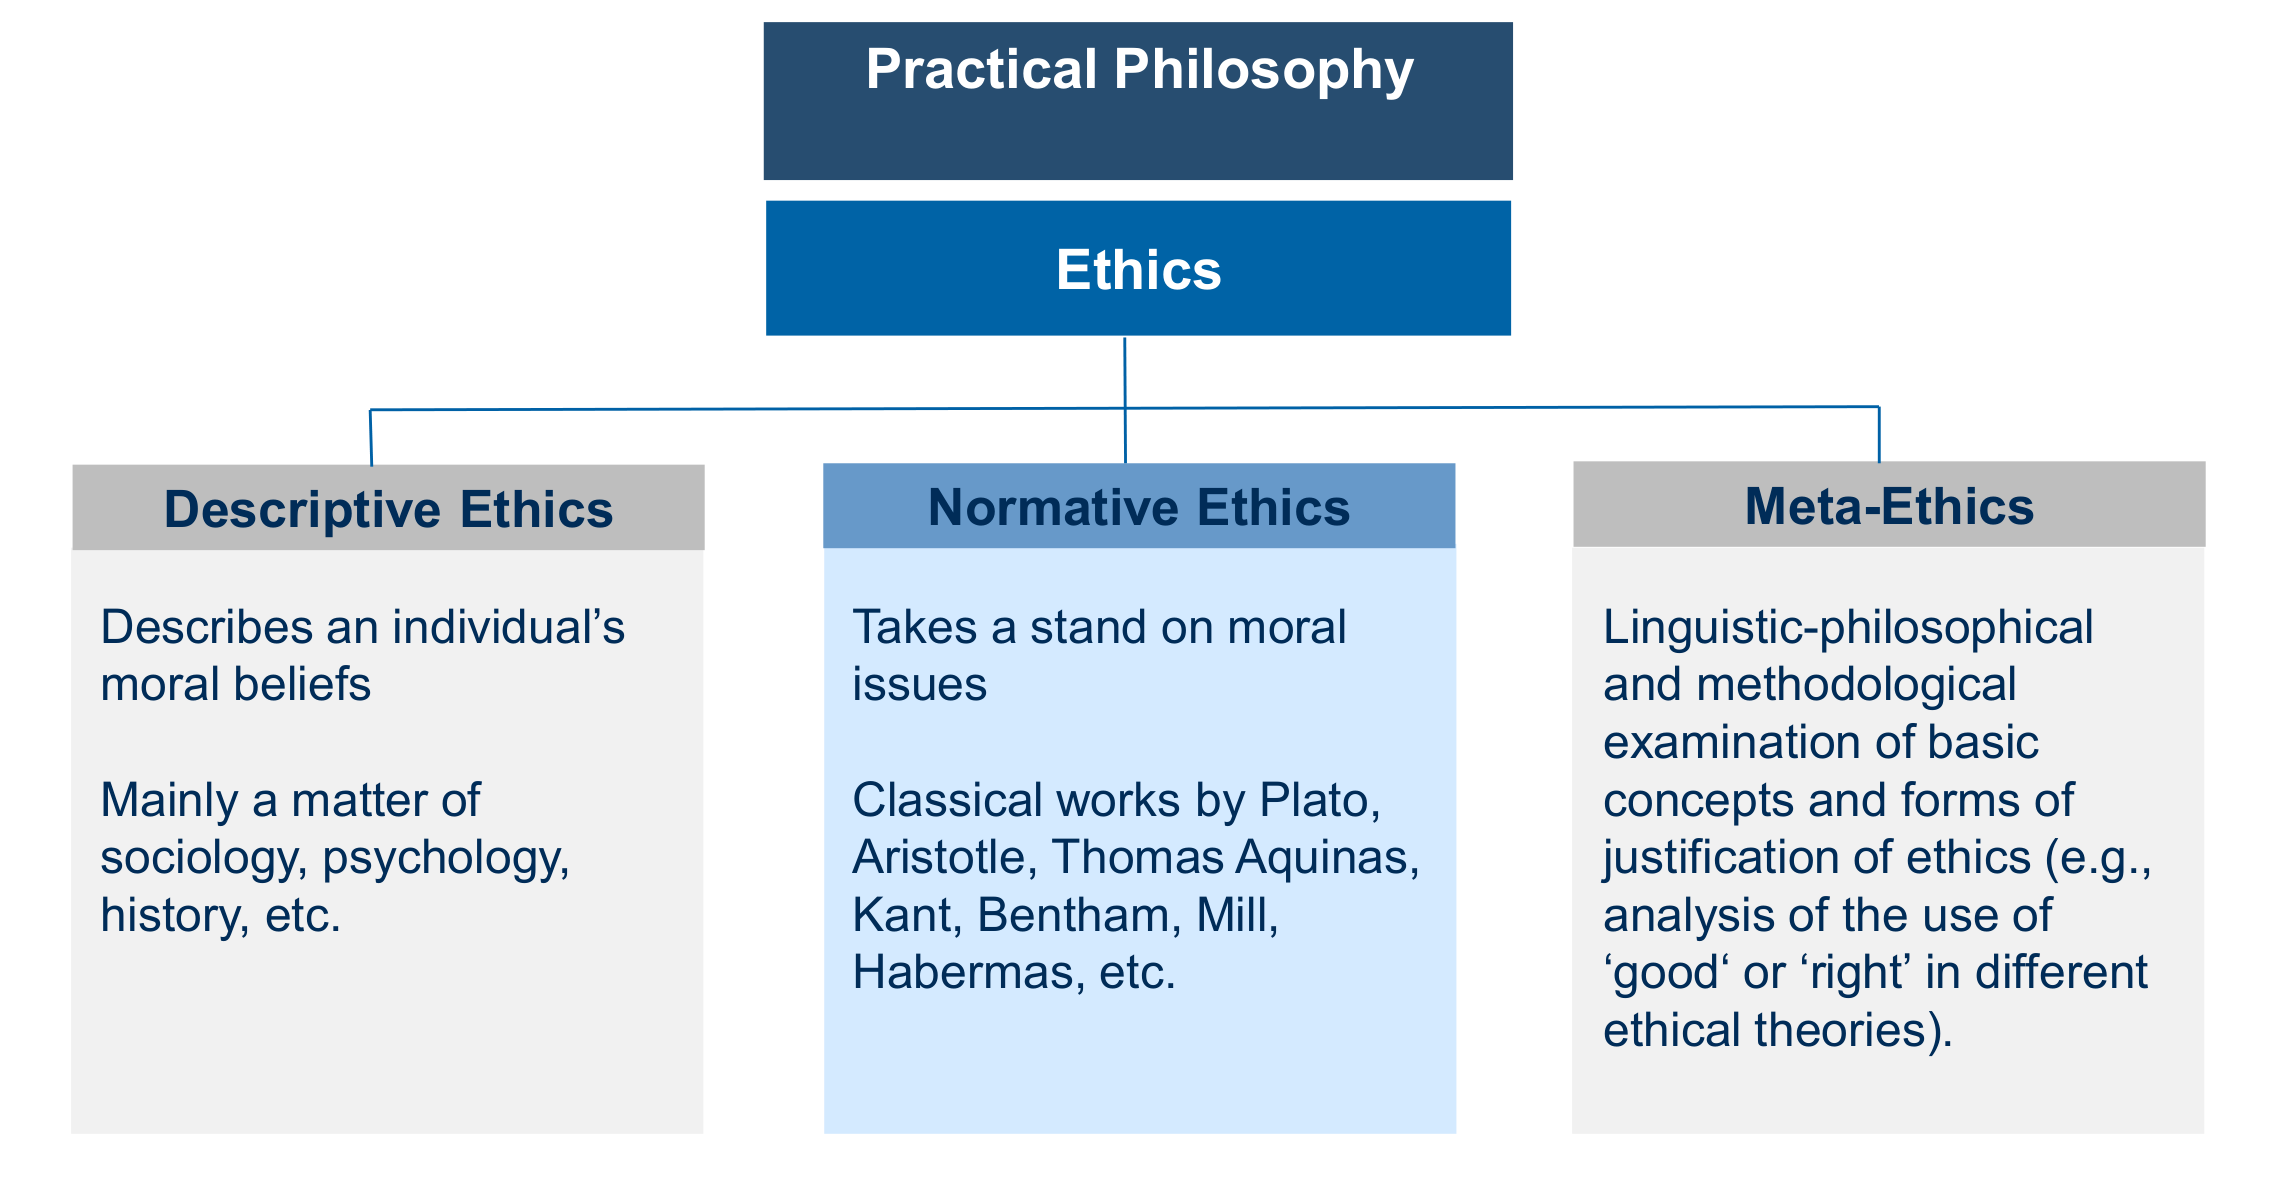
\includegraphics[width=0.8\linewidth]{img/classification_ethics}
	\caption{Classification of ethics}
	\label{fig:classificationethics}
\end{figure}

\section{Virtue Ethics}
Virtue ethics is an ethical mindset that places the emphasis of moral judgment on the motivation for human behaviour. This can either be an isolated thought that prevails at a given moment and causes a particular action to be taken. Or it can be a permanent attitude that develops over time and shapes an individual’s conduct over an entire life \parencite{hubner2018einfuhrung}.

Different virtue ethics focus on the motivation for human action. The actual actions of an individual or the consequences of these actions are not completely disregarded, but are not the prime object of moral judgement. Virtues are often defined in such a way that they strongly recommend an action or desirable consequences. Virtue ethicists do not make any strong recommendations regarding precise actions but are only concerned with the nature of these actions.

The main concepts rooted in ancient Greek philosophy are
\begin{enumerate}
	\item \emph{arête} - excellence or virtue
	\item \emph{phronesis} - practical or moral wisdom
	\item \emph{eudaimonia} - translated as happiness or flourishing
\end{enumerate}

\subsection{Plato's Parts of the Soul and His Virtues}
Plato was the first to really think about these aspects and write it down!
\begin{tabularx}{\linewidth}{|l|l|}
	\hline
	\textbf{Virtue} & \textbf{Connection to the Parts of the Soul}\\
	\hline
	Prudence & Reason (rulers) recognizes the appropriate course of action for the soul \\
	Fortitude & Courage (guardians) persists in what has been recognized through reason. \\
	Temperance & All parts of the soul (all citizens) agree that reason (rulers) should rule. \\
	Justice & Every part of the soul contributes (is met if the three other virtues prevail) \\
	\hline
\end{tabularx}

\subsection{Nicomachian Ethics}
Virtue of thinking needs teaching, experience and time, virtue of character (moral virtue) comes about as a consequence of following the right habits. According to Aristotle the potential for this virtue is by nature in humans, but whether virtues come to be present or not is not determined by human nature.

For Aristotle virtues are \textbf{positive}, \textbf{medium character traits} which must be in line with the nature of people, and their actions should be guided by \textbf{reason} and \textbf{insight}.

\begin{definition}
	A \textbf{theological concept} states that if an individual in a community behaves according to the virtue doctrine, he or she will lead a happy life and be considered ethical.
\end{definition}

According to Aristotle the \textbf{highest good} is \textquotedblleft living well\textquotedblright, to always strive for a good life for its own sake. \textbf{Good behaviour is, therefore, the moral goal,} and the highest goal can only be realized in the behaviour itself.

It must be the highest goal of human behaviour to realize reasonableness to the highest degree. Happiness, therefore, consists in acting according to a highly developed reason. This reason is, however, only highly developed if it is of a virtuous nature. Acting out of virtue or virtuous action by the human soul is the highest goal (\textbf{eudaimonia}).

Aristotle distinguishes between two categories of virtue
\begin{tabularx}{\linewidth}{l @{\hskip 2cm} l}
	\textbf{Intellectual} & \textbf{Ethical}\\
	\hline
	Wisdom & Generosity \\
	Prudence & Considerateness \\
	Perception & Courage \\
\end{tabularx}

\subsubsection{Criticism of Aristotelian Ethics}
\begin{itemize}[label=-]
	\item Aristotelian ethics cannot make concrete recommendations
	\item Aristotelian ethics is too relative
	\item The virtuous life does not always lead to a happy life
\end{itemize}

\subsection{Exercise Answers}
% TODO Correct the answers
\begin{enumerate}
	\item \textbf{What are the three normative approaches introduced in the text?}\\
	The meaning of virtue itself (arête), practical wisdom on how to act virtuous (phronesis), and the goal of using virtuous behaviour (eudaimonia)
	\item \textbf{How is virtue ethics distinguished from the two others?}\\
	Virtue ethics in contrast to an ethical approach focussing on rules (deontology) and the approach focussing on the consequences of actions (consequentialism) focusses on the behaviour or intent of the individual acting virtuous. A virtuous individual is not just so by virtue itself, but has a virtuous mind which lets the person act in a virtuous way in any circumstance, and with ease. Thus such an individual is said to posses "full or perfect virtue" in contrast to a person which has to control his impulses to act virtuous.
	\item \textbf{How is arête (excellence or virtue) defined in the text?}\\
	As a character trait which enables an individual to act in a virtuous manner. 
\end{enumerate}

\section{Deontological Ethics}
Deontological Ethics, \textit{deon} meaning \textquotedblleft obligation\textquotedblright\ in Greek, try to answer the question which norms and actions a person should do to be ethical. The most representative of a deontological approach is by Immanuel Kant:
\begin{itemize}[noitemsep]
	\item The goal of ethics is the observance of what is ethically correct
	\item The ethically good depends on the ethically correct
	\item The ethically correct is independent of the consequences
\end{itemize}

\begin{definition}
	\textbf{Duty} is an action to which a person is obliged. \parencite{kant1870grundlegung}
\end{definition}

\begin{definition}
	\textbf{The Categorical Imperative} is to act as if the maxims of your behaviour could, through your will, serve at any time as the basis of a general law. \parencite{kant1870grundlegung}
\end{definition}

\begin{definition}
	\textbf{Morality} is to do what is your duty (to follow absolutely valid norms of action) and do it out of duty (with a moral attitude).
\end{definition}

\subsection{Kant's Deontological Ethics}
Kant's deontological ethics are based on the idea that only free will that rules an autonomous action determines the ethical quality of an action, and that every individual has dignity and a free will. As a result, only the responsibility for actions resulting from freedom to act or autonomy can be judged ethically.

Kant's conception of freedom is to act freely, that is to act autonomously and guided by a law given by the individual itself. The opposite of autonomy is heteronomy, that is to act according to desires the individual has not chosen itself. While the value of an action can only be measured by the intention behind it, the quality of this intention can only be judged by the \textbf{action maxim} chosen by the subject. This capacity to act freely is what gives human lives its special dignity, and to respect this dignity means regarding people not just as a means to an end but as ends in themselves.

\subsection{The Categorical Imperative}
An action is morally correct if it follows maxims which are good in themselves.
\begin{enumerate}
	\item Act only according to a maxim according which you can also want it to become a universal law
	\item Act as if the maxims of your behaviour could, through your will, serve at any time as the basis of a universal law of nature
	\item Act as if you always need humanity, both in yourself and in the person of everyone else, as an end in itself, never merely as a means to an end
\end{enumerate}

\subsection{Human Rights}
Human rights are basic rights and every human being is entitled to them by nature. These rights apply \textbf{regardless of place and time} and are codified in the United Nations Universal Declaration of Human Rights (1948).

\subsection{Principles of Discourse Ethics}
\begin{itemize}
	\item Communicative action as a referential framework for the lifeworld of a society
	\item Solving conflicts by means \textbf{non-violent communication} and with \textbf{rational arguments}
	\item \textbf{Human rights} as basis
	\item In an ideal, practical discourse all those involved participate and agree to a norm in the end
	\item Reasons must be given, Fairness and Consequences
\end{itemize}

\begin{figure}[tbh]
	\centering
	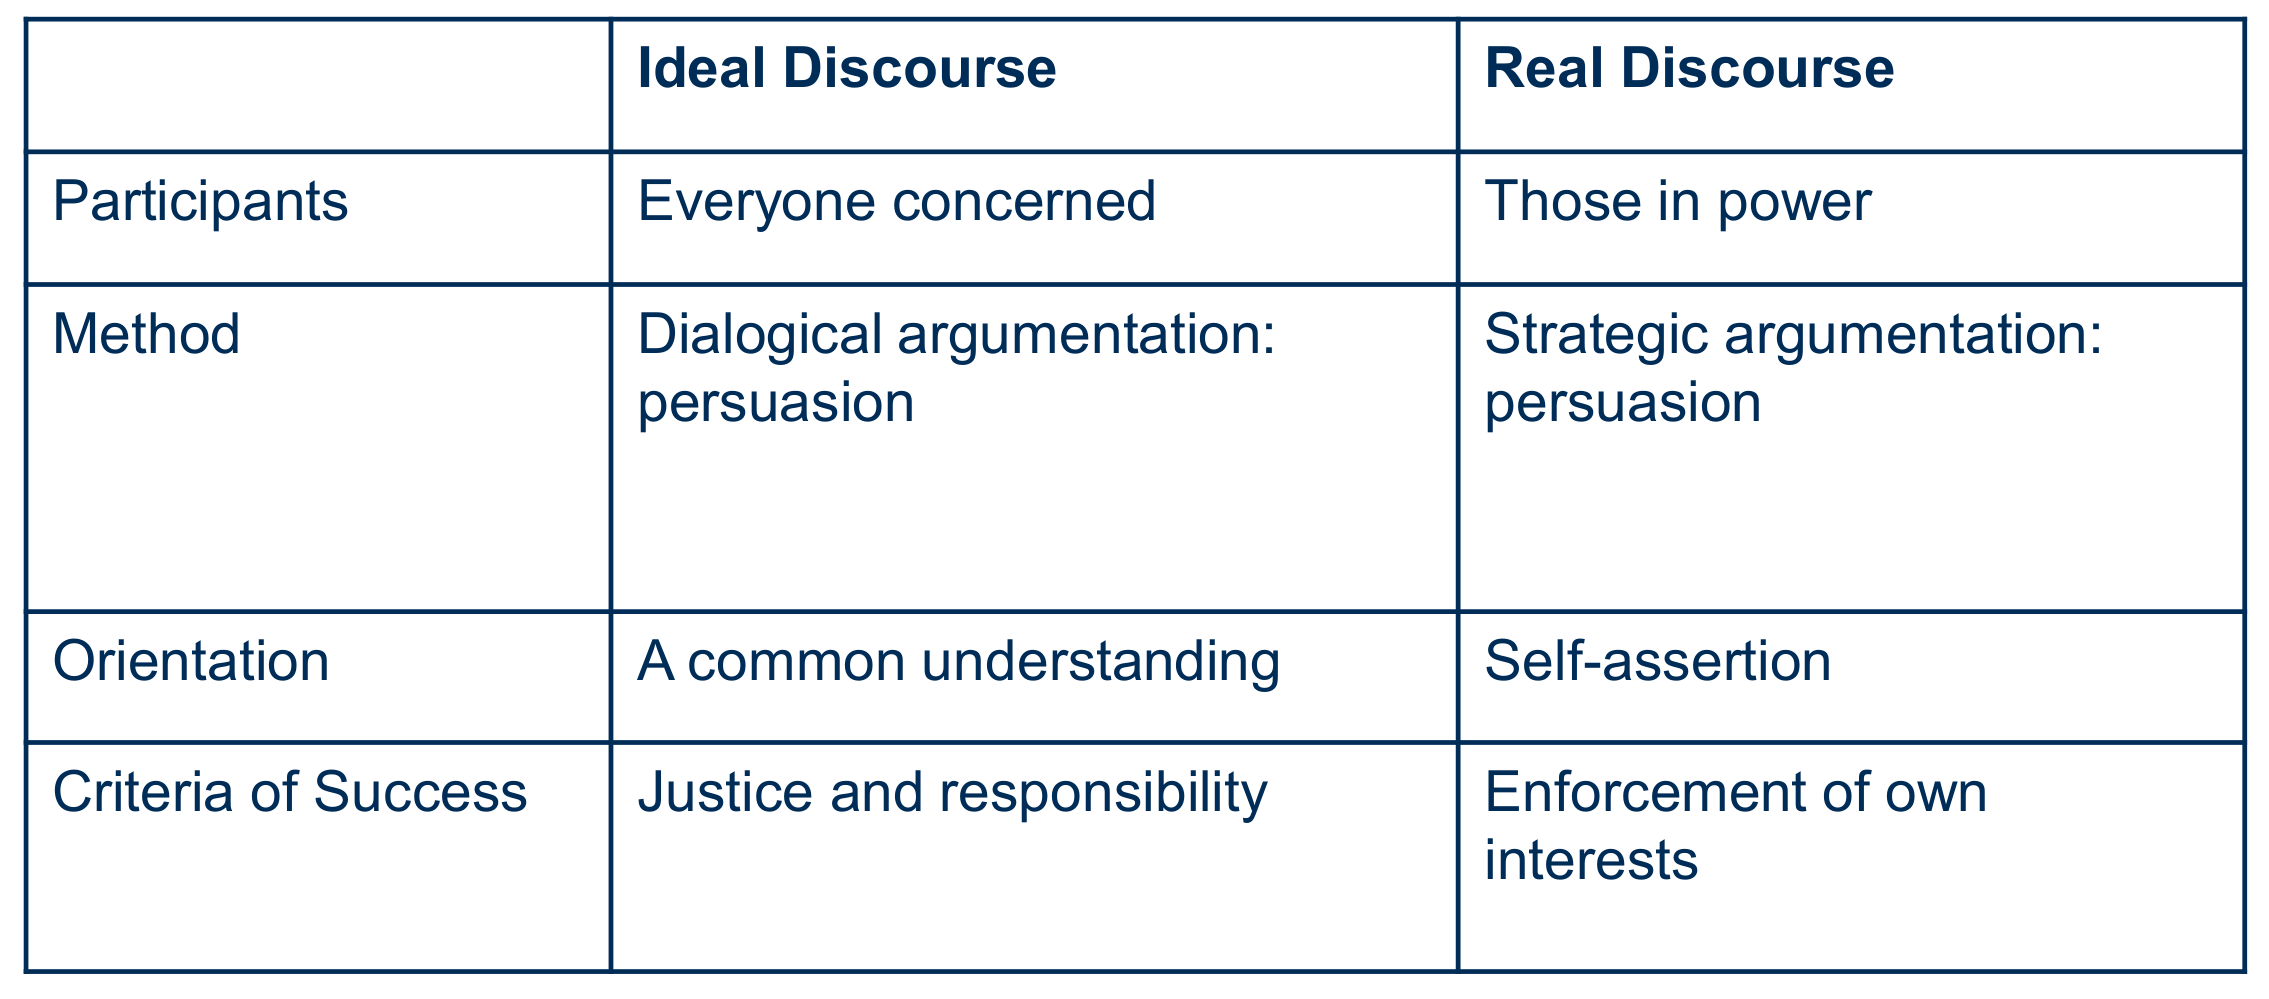
\includegraphics[width=0.8\linewidth]{img/discourse_comparison}
	\caption{Comparison between an ideal discourse and how real discourses often take place}
	\label{fig:discoursecomparison}
\end{figure}

\subsection{A Theory of Justice}
% TODO Read Rawls
The original position is the contract-theoretical justification of principles. Justice should be fairness, and there is a principle of impartiality or a "veil of ignorance".

Principles
\begin{enumerate}
	\item Each person has the same indefeasible claim to a fully adequate scheme of equal basic liberties, which scheme is compatible with the same scheme of liberties for all;
	\item Social and economic inequalities are to satisfy two conditions:
	\begin{enumerate}
		\item They are to be attached to offices and positions open to all under conditions of fair equality of opportunity;
		\item They are to be to the greatest benefit of the least-advantaged members of society (the difference principle; according to the MaxMin principle in game theory)
	\end{enumerate}
\end{enumerate}

\subsection{Exercise Answers}
\begin{enumerate}
	\item What are weaknesses of the deontological approach?
\end{enumerate}

%%% BIBLIOGRAPHY %%%

\printbibliography

\end{document}
